\chapter{Theory}

To understand the function of an optical dipole-trap one has to understand how far detuned light, more specificly the electric field component, interacts with a neutral atom. There are several models providing different levels of accuracy for the respective application. The atom can be treated rather classically by regarding it as a harmonic oscillator driven by an electric field. It can be treated semiclassically by considering the quantum nature and structure of the atom while still approximate the incoming light as electromagnetic waves. In this model the problem can be solved in second-order pertubation theory. The third approach is treating the atom quantum mechanically as well as the light, now consisting of quantised photons interacting with the atom. For this thesis only the first two approaches are relevant. 

\section{The Hamiltonian}

The problem of interaction between an atom, laser-light and in the case of this experiment also magnetic fields is represented by different parts in the total hamiltonian. The basis for all calculations is the atomic hamiltonian of the regardet Lithium-atoms $H_A$. The atom-light-interaction is represented by the Hamiltonian of the light itself $H_L$ and the interaction Hamiltonian $H_{AL}$ while the last contribution is the magnetic field Hamiltonian $H_M$.
\begin{equation}
H=H_A+H_L+H_{AL}+H_{M}
\end{equation}\label{hamiltonian}

\section{Lithium Level-structure}
The atomic hamiltonian $H_A$ coresponds to the energy of the atomic species that is used in our experiment, which is Lithium-6. Lithium is a fermionic alkali-metal, whose electronic structure is mostly dependent of its one valence electron \cite{gehm}. In this approximation, the \textit{central-field approximation}, the two other bound electrons on the most inner level only contribute to the central electric field, that is suppost to be sphericaly symetric. Thus the calculation can follow the well understood model of hydrogen. The ansatz in this case is considering an elelctron with the reduced mass $\mu$ in a coulomb-potential.
\begin{equation}
U(\boldsymbol{r})=-\frac{e^2Z}{4\pi\epsilon_0\boldsymbol{r}}
\end{equation}
That leads to the Hamiltonian:
\begin{equation}
H_A=\frac{p^2}{2\mu}-\frac{e^2Z}{4\pi\epsilon_0\boldsymbol{r}}
\end{equation}
Solving the Schrödinger-Equation considering this Hamiltonian leads to a set of wave-functions characterized by the quantum numbers $N,L,m_L$, $N$ being the main quantum number, $L$ the angular momentum quantum number and $m_L$ the projection onto the coordinate axis. The energy-levels for different $L$ are degenerate, but when the spin of the valence electron is considered this degeneracy is broken and the coupling of this spin to the orbital angular momentum leads to the fine-structure picture in which $J=l\pm S$  and $m_J=J,J-1,\dots,-J+1,J$ are the respective quantum numbers.
\begin{figure}[H]
\begin{center}
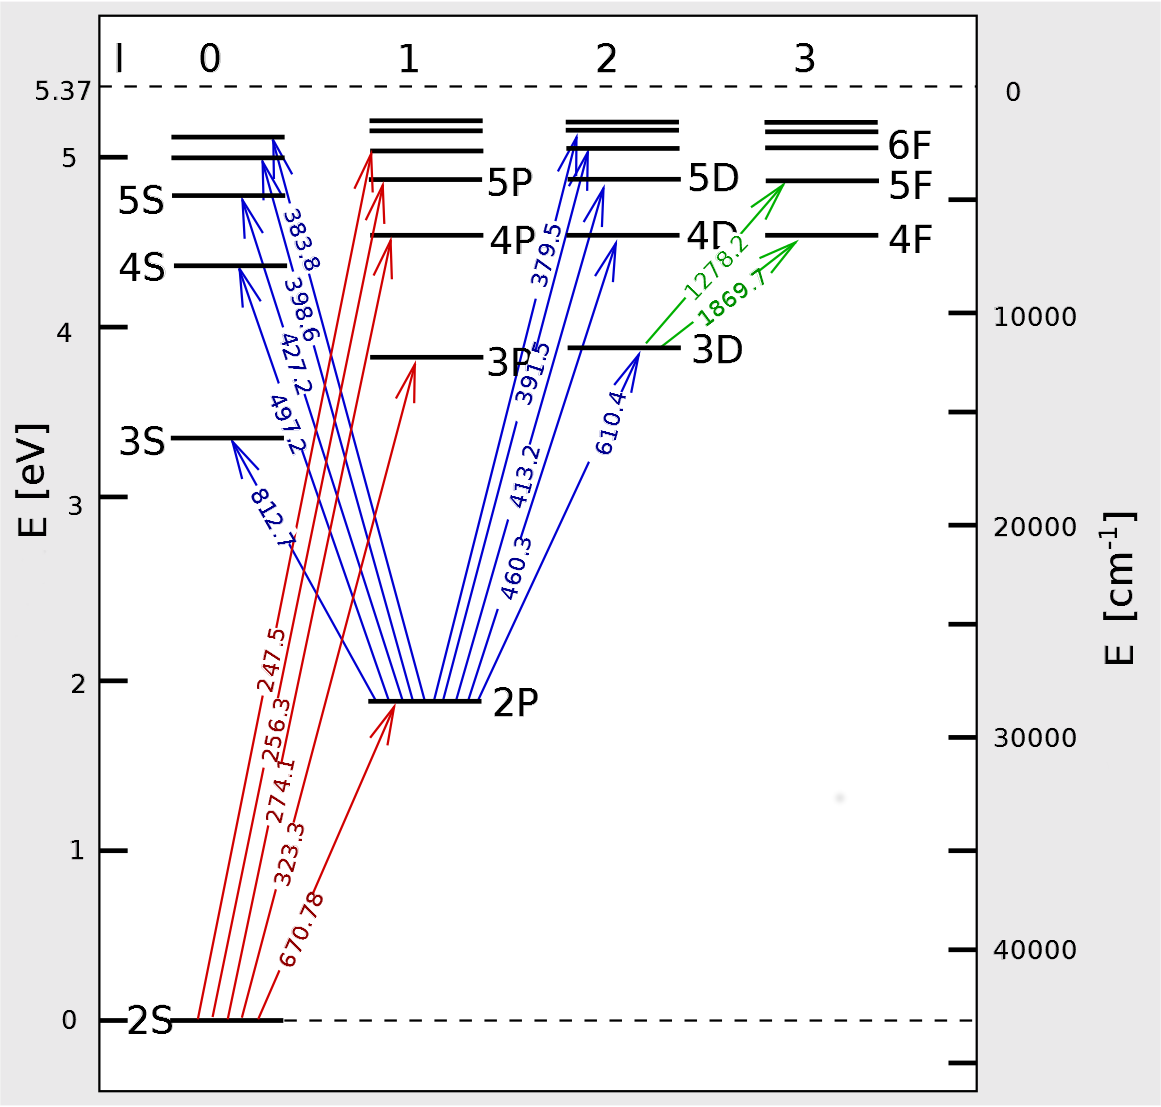
\includegraphics[scale=.4] {levels2}
\end{center}
\caption{Level structure of Lithium with the respective transitions, according to selection rules \cite{transitions}.}
\label{levels2}
\end{figure}
Nevertheless the real Lithium-atom has a substructure arising from interaction of the spin of the core with the angular momentum of the orbit. This effect results in the hyperfinestructure that breaks the degeneracy of the levels with same quantum number $J$. In the picture of hyperfinestructure the total angular momentum and the spin of the core $I$ couple to the new total angular momentum $F=J\pm I$ with their respective projections $m_F=F,F-1,\dots,-F+1,F$ that result in a even finer splitting of the lines, and fully characterize a lithium-atom.

\begin{figure}[H]

\begin{center}
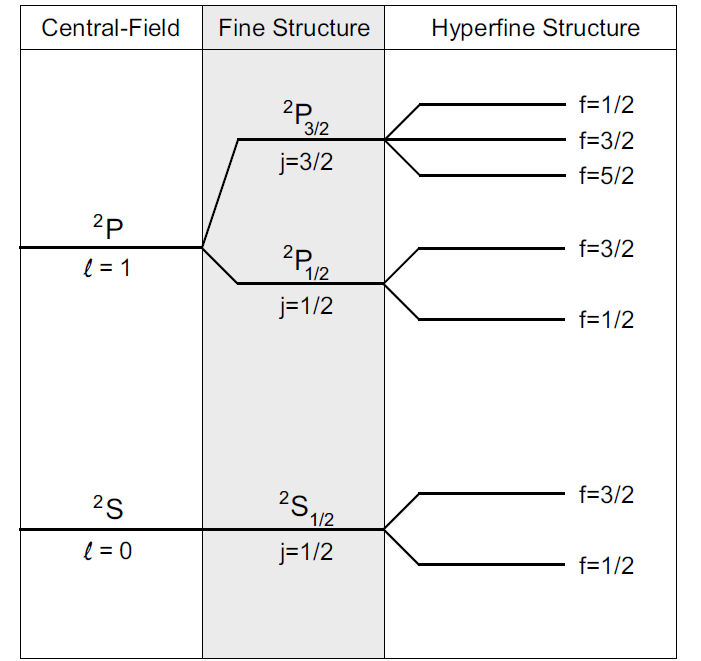
\includegraphics[scale=.5] {levels1}
\end{center}
\caption{Extract of the level structure for Lithium-6 in the fine and hyperfine regime \cite{gehm}}
\label{levels1}
\end{figure}

\section{Magnetic Field}

Within the experiment, the regarded atoms are exposed to strong magnetic fields. Therefore, additionally the Zeeman-Effect moves the respective levels contributing to the \textsc{ac}-Stark-Shift. In this approach we simply regard both effects as independent pertubations to the basic Hamiltonian. At strong magnetic fields, as used in the experiment, the Paschen-Back-Effect for hyperfine states dominates and instead of $F$ and $m_F$, the quantum numbers $J$ and $m_J$ are still “good“. Therefore the formula for the shift of each state is given by:
\begin{equation}
\Delta E=g_Jm_j\hslash\gamma B
\end{equation}
With $\gamma=e/(2m_e)$ and $g_J$ being the Landé-factor. The results are new values of energy-difference i.e. detuning for the respective transitions that now have a different contribution to the \textsc{ac}-Stark-Effect. 

\newpage
\newpage
\section{AC-Stark-Shift}
The \textsc{ac}-Stark-Shift arises from the interaction of electric fields with the regarded atom. Before treating this problem quantum-mechanicaly in terms of our Hamiltonian (\ref{hamiltonian}), we look at the problem in a classical model, that already results in a formula, that is very accurate in certain systems. 
\subsection{Lorentz Oscillator Model}

 Classicaly the problem of light-matter-interaction can be described in terms of an atomic dipole moment induced by an oscillating electric field, following \cite{dipole}. The atom is hereby described as a damped harmonic ocillator driven by the field. Intuitively one can think of the electrons and the core being pulled away from each other by the electric force, resulting in an oscillation against each other. The potential arising from these conditions is the following\footnote{The force on a dipole is given by \cite{factor}:
\begin{equation*}
\boldsymbol{F}=(\boldsymbol{p}\cdot\nabla)\boldsymbol{E}
\end{equation*}
We know that the following holds:
\begin{equation*}
\nabla(\boldsymbol{p}\cdot\boldsymbol{E})=\boldsymbol{p}\times(\nabla\times\boldsymbol{E})+\boldsymbol{E}\times(\nabla\times\boldsymbol{p})+(\boldsymbol{p}\cdot\nabla)\boldsymbol{E}+(\boldsymbol{E}\cdot\nabla)\boldsymbol{p}
\label{dipoleforce}\end{equation*}
We consider the trap to consist of a retro-reflected laserbeam, that is in phase, so the B-field-component of the electromagnetic wave is onsidered to be 0 as well as $\nabla\times\boldsymbol{E}=-\partial\boldsymbol{B}/\partial t=0$. In our case the dipole-moment is not constant but \(\boldsymbol{p}=\alpha \boldsymbol{E}\) and thus becomes:
\begin{equation*}
\nabla(\boldsymbol{p}\cdot\boldsymbol{E})=\alpha\boldsymbol{E}\times(\nabla\times\boldsymbol{E})+\alpha\boldsymbol{E}\times(\nabla\times\boldsymbol{E})+(\alpha\boldsymbol{E}\cdot\nabla)\boldsymbol{E}+\alpha(\boldsymbol{E}\cdot\nabla)\boldsymbol{E}
\end{equation*}
which becomes:
\begin{align*}
\nabla(\boldsymbol{p}\cdot\boldsymbol{E})&=2\alpha(\boldsymbol{E}\cdot\nabla)\boldsymbol{E}=2(\boldsymbol{p}\cdot\nabla)\boldsymbol{E}\\
\Rightarrow \boldsymbol{F}&=\frac{1}{2}\nabla(\boldsymbol{p}\cdot\boldsymbol{E})
\end{align*}
To get the corresponting potential one has to integrate the force. For a rapidly oscillating field we futher have to take the time average to get an effective value for the trapping potential.
\begin{equation*}
U=-\frac{1}{2}\mean{\boldsymbol{p E}}
\end{equation*}}:
\begin{equation}
U=-\frac{1}{2}\mean{\boldsymbol{p E}}
\label{dipole}
\end{equation} 
Here $\boldsymbol{p}$ is the induced dipole moment, $\boldsymbol{E}$ the electric field. The time-average is introduced since the electric field in an electro-magnetic wave is oscillating very fast and the atom “feels“ an effective potential averaged over the oscillation. If we only consider the real part of $\boldsymbol{p}\boldsymbol{E}\propto \cos^2$, the time average is $\mean{\boldsymbol{p}\boldsymbol{E}}=1/2 \mathrm{ Re}(\alpha)E^2$. One can rewrite (\ref{dipole}) in terms of the Intentity $I=1/2\epsilon_0cE^2 $:
\begin{equation}
U=-\frac{1}{2\epsilon_0 c}\mathrm{Re}(\alpha)I
\end{equation} 

To calculate the exact potential one has to obtain a value for $\alpha$. In this classical description an electron is considered bound to the core elastically with the oscillation eigenfrequency $\omega_0$ corresponding to the optical transition frequency. In our practical case that is the frequency of the Lithium-D2-Line. In a real atom, there are of course multiple resonances, corresponding to multible states of the electron, thus this is approximation yields only for certain cases in which the system can also be regarded as a quantummechanical two-state-system. We will later see, that while this approach leads to a very accurate calculation for the Lithium ground state, it can not at all be applied to the calculation of the trapping potential for the first excited state, since there exists no single dominant transition, but multiple resonances, all contributing to the respective energy-shift, in contrast to the groundstate.

The polarizability now can be calculated by solving the equation of motion of a driven and damped harmonic oscillator.
\begin{equation}
\ddot x+\Gamma_\omega\dot x+\omega^2_0x=-\frac{eE(t)}{m_e}
\end{equation} 
for that the solution can be calculated using basic tools for differential-equation-solving. The result is then:
\begin{equation}
\alpha=\frac{e^2}{m_e}\frac{1}{\omega^2_0-\omega^2-\mathrm{i}\omega\Gamma_\omega}
\end{equation} 
With
\begin{equation}
\Gamma_\omega=\frac{e^2\om^2}{6\pi\epsilon_0m_ec^3}
\end{equation}
We can substitute $e^2/m_e=6\pi\epsilon_0c^3\Gamma_\omega/\om^2$ and define the on-resonance damping rate $\Gamma:=(\om_0/\om)^2\Gamma_\omega$ witch results in the form:
\begin{equation}
\alpha=6\pi\epsilon_0c^3\frac{\Gamma/\om^2_0}{\omega^2_0-\omega^2-\mathrm{i}(\om^3/\om^2_0)\Gamma}
\end{equation} 
We now can plug the real part of this expression in (\ref{dipole}) and obtain the very known formula:
\begin{equation}
U_{dip}(\boldsymbol{r})=-\frac{3\pi c^2}{2\om^3_0}(\frac{\Gamma}{\om_0-\om}+\frac{\Gamma}{\om_0+\om})I(\boldsymbol{r})
\label{classic}\end{equation}
In this case, the damping parameter $\Gamma$ corresponds to the linewidth of the optical transition, which numerical value is $\Gamma=5.8724 \unit{MHz}$ for the considered D2-Line \cite{gehm}.

\subsection{Energy-Shift in Pertubation Theory}

After this classical treatment, we come back to calculating the same effect quantum-mechanically. For calculating the energy-shift for the first excited state, this is the only way to get a trustworthy result since in contrast to the ground state of Lithium it can not be approximated by a two-level-system with only one transition. Therefore we have to solve the problem more precicely. 

The interaction of the atom with laser-light is described by the two additional parts in the original hamiltonian (\ref{hamiltonian}) $H_L+H_{AL}$. The light-hamiltonian $H_L$ is hereby negligible, because the regarded laser-light of the used dipole-trap is farly detuned from the relevant transition resonances. Therefore the only relevant part of this set of terms is the interaction-hamiltonian, which depends on the dipole-operator $\mu$ and the electric-field-operator $E$ and has the following form: $H_{AL}=-\mu E=-e\boldsymbol{r} E$. It can be treated as a small pertubation of the atomic hamiltonian, thus in the relevant second-order pertubation-theory the energy-shift is the following \cite{dipole}:
\begin{equation}
\Delta W=\sum_{k\neq j}\frac{|\braopket{j}{H_{AL}}{k}|^2}{W_k-W_j}
\label{pertub1}
\end{equation}
Although the hyperfine splitting is highly relevant for the experiment itself, it is sufficient for the calculation of the Stark-Shift to only consider the fine-structure regime. Aspecially at high-strength magnetic fields, the hyperfine Paschen-Back-Effect leads to degeneracy of the different hyperfine states and the total angular momentum $J$ is a "good quantum-number" again. In the low-field-regime the corrections due to hyperfine-splitting are small, because of the little energy-differences compared to the relevant transitions between the levels in the fine-structure-regime and the considered large detuning of the dipole-trap-light. Hence also there this picture is sufficient. In this case (\ref{pertub1}) can be expressed in terms of $J$ and $m_J$ and with the explicit form of $H_{AL}$ this becomes\cite{alpha}:
\begin{equation}
\Delta W_{Jm_j}=-e^2\sum_{K\neq J}\sum_{m_k}\frac{\braopket{Jm_J}{\boldsymbol{r}E}{Km_K}\braopket{Km_K}{\boldsymbol{r}E}{Jm_J}}{W_k-W_j}\boldsymbol{r}E\label{pertub2}
\end{equation}
The main problem now is to calculate the coupling of different angular momenta. That is why most of the calculation is dedicated to simplify the calculation of all relevant Clebsch-Gordan coefficients.\\\\
We will now describe the electric field in terms of irreducible tensor operators:
\begin{align}
E_{\pm}=\mp\frac{1}{2}\sqrt{2}(E_x\pm \mathrm{i}E_y),\ \ \ E_0=E_z\\
r_{\pm}=\mp\frac{1}{2}\sqrt{2}(r_x\pm \mathrm{i}r_y),\ \ \ r_0=r_z\\
\end{align}
In this notation we can rewrite (\ref{pertub2}) in terms of these operators:
\begin{equation}
\Delta W_{Jm_j}=-e^2\sum_{K\neq J}\sum_{m_k}\sum_{\mu\nu}(-1)^{\mu+\nu}E_\mu E_\nu\frac{\braopket{Jm_J}{r_{-\mu}}{Km_K}\braopket{Km_K}{r_{-\nu}}{Jm_J}}{W_k-W_j}\label{pertub3}
\end{equation}
With $\mu=0,\pm1$. Now, we define the following sum, that will be used later on. Note that is a simple shorting for simplification.
\begin{equation}
\mathcal{E}(L,m_L):=\\sum_{\mu\nu}\sqrt{2L+1}(-1)^{m_L}\threej{1}{1}{L}{\mu}{\nu}{-m_L}E_\mu E_\nu\label{irreducible}
\end{equation}
We here also use the Wigner 3-j-symbol-notation\footnote{The Wigner 3-j symbol and 6-j symbol are definded in terms of Clebsch-Gordan-Coefficients:\begin{align}\threej{j_1}{j_2}{j_3}{m_1}{m_2}{m_3}:=&\frac{(-1)^{j_1-j_2-m_3}}{\sqrt{2j_3+1}}\braket{j_1m_1j_2m_2}{j_3-m_3}\\\sixj{j_1}{j_2}{j_3}{j_4}{j_5}{j_6}:=&\sum^6_{m_j}(-1)^{\sum^6_{k=1}(j_k-m_k)}\threej{j_1}{j_2}{j_3}{m_1}{m_2}{-m_3}\threej{j_1}{j_5}{j_6}{-m_1}{m_5}{m_6}\\\times&\threej{j_4}{j_5}{j_3}{m_4}{-m_5}{m_3}\threej{j_4}{j_2}{j_6}{-m_4}{-m_2}{-m_6}\label{jsymbols}\end{align}}. Therefore we can write the product in (\ref{pertub3}) in terms of this sum: 
\begin{equation}
E_\mu E_\nu=\sum^2_{L=0}\sum^L_{m_L=-L}\sqrt{2L+1}(-1)^{m_L}\threej{1}{1}{L}{\mu}{\nu}{-m_L}\mathcal{E}(L,m_L)
\end{equation}
For later-on simplification, we can calculate (\ref{irreducible}) explicitly for different combinations of $L$ and $m_L$.
\begin{align*}
\mathcal{E}(0,0)&=-\frac{1}{\sqrt{3}}(E^2_0-2E_{-1}E_{1})=-\frac{1}{\sqrt{3}}(E^2_z-2(-\frac{1}{2}(E_x+\mathrm{i}E_y)(E_x+\mathrm{i}E_y))\\&=-\frac{1}{\sqrt{3}}(E^2_z+E²_x+E^2_y)=-\frac{1}{\sqrt{3}}E^2\\
\mathcal{E}(1,\pm 1)&=0\\
\mathcal{E}(1,0)&=0\\
\mathcal{E}(2,\pm2)&=E^2_{\pm1}=\frac{1}{2}(E_x\pm \mathrm{i}E_y)^2\\
\mathcal{E}(2,\pm1)&=(E_x\pm \mathrm{i}E_y)E_z\\
\mathcal{E}(2,0)&=\sqrt{\frac{2}{3}}(E^2_0+E_{-1}E_1)=\sqrt{\frac{2}{3}}(E^2_z+\frac{1}{2}E^2_z-\frac{1}{2}E^2_z-\frac{1}{2}(E^2_x+E^2_y))\\&=\frac{1}{\sqrt{6}}(3E^2_z-E^2)
\end{align*}
After finishing that horrible calculation, the next step is to evaluate the sum in (\ref{pertub3}), which is even more terrifying, as you can imagine!

The first step is to evaluate the inner part, that is the summation over the respective magnetic quantum numbers $m_J$. Thus we give it an own name and define:
\begin{equation}
\mathcal{S}(J,m_J)=\sum_{m_k}\sum_{\mu\nu}(-1)^{\mu+\nu}E_\mu E_\nu\braopket{Jm_J}{r_{-\mu}}{Km_K}\braopket{Km_K}{r_{-\nu}}{Jm_J}\label{sum}
\end{equation}
The matrix elements can be calculated using the Wigner-Eckart theorem\footnote{The Wigner-Eckart theorem simplifies the calculation of matrix-elements in a spherical basis and breaks it down to the calculation of few reduced matrix elements. For an irreducible tensor-operator $T^r_q$ between two angular-momentum eigen-states the following holds \cite[17]{wigner}:
\begin{equation}
\braopket{j,m_j}{T^r_q}{k,m_k}=\braopket{j}{|T^r|}{k}C^{jm_j}_{rqkm_k}
\end{equation}
In this formula $r$ denotes the rank of the tensor, and $q$ is simply the respective component of the tensor. Writing this in terms of the 3-j symbols yields:
\begin{equation}
\braopket{j,m_j}{T^r_q}{k,m_k}=(-1)^{j-m_j}\threej{j}{r}{k}{-m_j}{q}{m_k}\braopket{j}{|T^r|}{k}
\end{equation}
The resulting reduced matrix elements are independent of the respective component of the operator and the $m$-quantum-number. Therefore for every pair of angular-momentum quantum numbers $j$ and $k$ only one reduced matrix element has to be calculated to evaluate all elements of eigenstates involving said angular momenta.}.
\begin{align}
\mathcal{S}(J,m_J)=&(-1)^{J-K}|\braopket{J}{|r|}{K}|^2\times\notag\\&\sum_L\sqrt{2L+1}\sum_{m_L}\mathcal{E}(L,m_L)\sum_{\mu\nu}(-1)^{\mu+\nu}(-1)^{m_L}\threej{1}{1}{L}{\mu}{\nu}{-m_L}\times\notag\\&\sum_{m_K}\left[(-1)^{J-m_J}\threej{J}{1}{K}{-m_J}{-\mu}{m_K}(-1)^{K-m_K}\threej{K}{1}{J}{-m_K}{-\nu}{m_J}\right]\label{sum2}
\end{align}
Note, that the first part of this term can be written in this way because because using the Wigner-Eckert theorem the tensor operator in the matrix element now has become the normal spherical coordinate-operator in the respective reduced matrix element, which of course is hermitian. The sum over $\mu,\nu$ and $m_K$ can be evaluated and rewritten in terms of the 6-j symbol.
\begin{align}
&\sum_{\mu\nu}(-1)^{\mu+\nu}(-1)^{m_L}\threej{1}{1}{L}{\mu}{\nu}{-m_L}\times\notag\\&\sum_{m_K}\left[(-1)^{J-m_J}\threej{J}{1}{K}{-m_J}{-\mu}{m_K}(-1)^{K-m_K}\threej{K}{1}{J}{-m_K}{-\nu}{m_J}\right]\notag\\&\ \ =(-1)^{2J}(-1)^{J-m_J}\threej{J}{L}{J}{-m_J}{0}{m_J}\sixj{J}{1}{K}{1}{K}{L}\delta_{m_L,0}
\end{align}
This, together with the values for $\mathcal{E}(L,m_L)$, leads to the fact, that only terms with $L=0,2$ and $m_L=0$ remain and the following holds:
\begin{align}
\mathcal{S}(J,m_J)=&(-1)^{J-K}|\braopket{J}{|r|}{K}|^2\times\notag\\&\sum_{L}\mathcal{E}(L,0)\sqrt{2L+1} (-1)^{J-m_J}\threej{J}{L}{J}{-m_J}{0}{m_J}\sixj{J}{1}{K}{1}{K}{L}\label{sum3}
\end{align}
Now, we arrive at the point, where we can go back to evaluating (\ref{pertub2}). The finding in (\ref{sum3}) means, that we can decompose $\Delta W_{Jm_J}$ into a sum over different $L$:
\begin{equation}
\Delta W_{Jm_J}=\sum_L\Delta W^L_{Jm_J}
\end{equation}
in which each of the components can be written, using the form of (\ref{sum3}).
\begin{align}
\Delta W^L_{Jm_J}=&-e^2\sum_{K\neq J}\frac{\braopket{J}{|r|}{K}|^2}{W_K-W_J}\mathcal{E}(L,0)\sqrt{2L+1}\notag\\&(-1)^{J+K} (-1)^{J-m_J}\threej{J}{L}{J}{-m_J}{0}{m_J}\sixj{J}{1}{K}{1}{K}{L}\label{pertub4}
\end{align}
For this equation we can analyse the only two different cases, namely for $L=0,2$. If we evaluate both components and use the values vor $\mathcal{E}(1,0)$ and $\mathcal{E}(1,0)$, we get to the both contributions to the energy-shift:
\begin{align}
\Delta W^0_{Jm_J}=&-e^2E^2\frac{1}{3(2J+1)}\sum_{K\neq J}\frac{\braopket{J}{|r|}{K}|^2}{W_K-W_J}\\
\Delta W^2_{Jm_J}=&-e^2(3E^2_z-E^2)\sqrt{\frac{5J(2J-1)}{6(2J+3)(J+1)(2J+1)}}\ \times\notag\\
&\frac{3m^2_J-J(J+1)}{J(2J-1)}\sum_{K\neq J}(-1)^{J+K}\sixj{J}{1}{K}{1}{J}{2}\frac{\braopket{J}{|r|}{K}|^2}{W_K-W_J}
\end{align}
We now chose the electric field to be directed along the z-axis: $\boldsymbol{E}=E\hat{\boldsymbol{z}}$ so we can say, that $E^2_z=E^2$. Thus follows:
\begin{align}
\Delta W^2_{Jm_J}=&-\frac{1}{2}e^2E^24C\ \times\notag\\
&\frac{3m^2_J-J(J+1)}{J(2J-1)}\sum_{K\neq J}(-1)^{J+K}\sixj{J}{1}{K}{1}{J}{2}\frac{\braopket{J}{|r|}{K}|^2}{W_K-W_J}\label{alpha21}
\end{align}
We are hereby shortening $C:=\sqrt{5J(2J-1)/6(2J+3)(J+1)(2J+1)}$.
Note, that if the z-direction also defines the quantisation axis in a magnetic field, this means assuming $\pi$-polarized laser-light. If the light is then supposed to be $\sigma$-polarized, the z-component has to be considered individually and is holds $E^2_z=1/2\ E^2$.
We now draw an analogy to the classical calculation and link the total energy-shift to the dipole potential by defining a polarizability, composed of the now defined scalar and tensor polarizability.
\begin{align}
\alpha:=&e^2\left[\alpha^0_J+\frac{3m^2_J-J(J+1)}{J(2J-1)}\alpha^2_J\right]\\
\notag\\
\alpha^0_J=&\frac{2}{3(2J+1)}\sum_{K\neq J}\frac{|\braopket{J}{|r|}{K}|^2}{W_K-W_J}\\
\alpha^2_J=&4C\sum_{K\neq J}(-1)^{J+K}\sixj{J}{1}{K}{1}{J}{2}\frac{|\braopket{J}{|r|}{K}|^2}{W_K-W_J}
\end{align}
An additional factor has to be multiplied in analogy to the classical formula. The electric field is oscillating and the average thus results in a factor of $1/2$, because we did not take the time into account, when calculating the polarizability.
\begin{align}
U=&-\frac{1}{2}\alpha E^2\notag\\
U=&-\frac{1}{4}e^2\left[\alpha^0_J+\frac{2m^2_J-J(J+1)}{J(2J-1)}\alpha^2_J\right]E^2\label{shift}
\end{align}

\section{Dipole Traps}

The \textsc{ac}-Stark-Shift, as described above can, as stated in the beginning, be used to trap neutral atoms. We so far have seen, that an electric field induces a dipole moment in the atom that leads to a dipole-potential.The resulting force is proportional to the gradient of the intensity-distribution around the atom, therefore to understand how a dipole trap works exactly, one has to study the properties of the applied beams. Lasers normally emmit gaussian beams. The intensitiy distribution along the radial profile at a given point on the course of the beam is \cite{dipole}:
\begin{equation}
I(r)=\frac{2P}{\pi w^2}\mathrm{exp}(-2\frac{r^2}{w^2})
\end{equation}
With $r$ being the radal coordinate, $P$ the power of the beam and $w$ the waist. In contrast to simle ray-optics, the focus of the gaussian beam is not point like but has a finite waist $w_0$. At this point the intensity of the focussed laser-beam is at its maximum:
\begin{equation}
I_{\mathrm{max}}=\frac{2P}{\pi w^2_0}
\end{equation}
This determines the deepest point in the potential, indepedent of the exact geometry of the trap, in case the center has a gaussian form. This is the case for both dipole-traps used in the experiment, that will be described in the next section.